\documentclass[11p, titlepage, oneside, a4paper]{article}
% Packages
\usepackage{amsmath}
\usepackage{graphicx}
\usepackage{hyperref}
\usepackage[english,swedish]{babel}
\usepackage[
    backend=biber,
    style=authoryear-ibid,
    sorting=ynt
]{biblatex}
\usepackage[utf8]{inputenc}
\usepackage[T1]{fontenc}
%Källor
\addbibresource{mall.bib}
\graphicspath{ {./images/} }

% Ändra de rader som behöver ändras
\def\inst{Teknikprogrammet}
\def\typeofdoc{Laborationsrapport}
\def\course{Fysik 1 150p}
\def\pretitle{Laboration 1}
\def\title{Rörelse: Hastighet och acceleration}
\def\name{Markus Glas och Alvin Granvik}
\def\username{magnus.glas}
\def\email{\username{}@elev.ga.ntig.se}
\def\graders{Magnus Silverdal}

\begin{document}

\begin{titlepage}
		\thispagestyle{empty}
		\begin{large}
			\begin{tabular}{@{}p{\textwidth}@{}}
				\textbf{NTI gymnasiet \hfill \today} \\
				\textbf{\inst} \\
				\textbf{\typeofdoc} \\
			\end{tabular}
		\end{large}
		\vspace{10mm}
		\begin{center}
			\LARGE{\pretitle} \\
			\huge{\textbf{\course}}\\
			\vspace{10mm}
			\LARGE{\title} \\
			\vspace{15mm}
			\begin{large}
				\begin{tabular}{ll}
					\textbf{Namn} & \name \\
					\textbf{E-mail} & \texttt{\email} \\
				\end{tabular}
			\end{large}
			\vfill
            
\includegraphics[width=0.5\textwidth]{images/NTI Gymnasiet_Symbol_print_svart.png}
			\vfill
            \large{\textbf{Handledare}}\\
			\mbox{\large{\graders}}
		\end{center}
	\end{titlepage}

    \begin{otherlanguage}{english}
	\begin{abstract}
		This report is about the velocity and acceleration of a cart on a tilted plane. The lab was made using a tilted plane a cart a program that meassures frame by frame and a ruler. It was performed by Markus Glas and Alvin Granvik and the results that were gathered are the following: The Cart traveled on a plane that had a negative distance, The cart traveled with a negative velocity and it accelerated negative aswell. These meassurements are off by so much because in the calculations in excel something messed up. The equations that were used were \begin{equation}
																																																																																																																																												   v_m = \frac{\Delta s}{\Delta t}
		\end{equation} and $a_m = \frac{\Delta v}{\Delta t}$ These equations calculate velocity and acceleration.
    \end{abstract}
    \end{otherlanguage}
    % Om arbetet är långt har det en innehållsförteckning, annars kan den utelämnas
	\pagenumbering{roman}
	\tableofcontents
	
	% och lägger in en sidbrytning
	\newpage

	\pagenumbering{arabic}
	
	% i Sverige har vi normalt inget indrag vid nytt stycke
	\setlength{\parindent}{0pt}
	% men däremot lite mellanrum
	\setlength{\parskip}{10pt}
	
	\section{Syfte och frågeställning}
		Syftet med laborationen är att beräkna hastighet och accelaration hos en vagn som rullar på en lutandes plan.

	\section{Bakgrund och teori}
        Med hjälp av ett program som mäter hastighet frame by frame vid vagnens olika tidpunkter kommer hastigheten och accelerationen räknas ut med formlerna $v_m = \frac{\Delta s}{\Delta t}$ för hastigheten och $a_m = \frac{\Delta v}{\Delta t}$ för accelartionen. Detta kommer ge aproxiemella värden för hastigheten och accelerationen som en funktion av tiden.


\section{Metod och materiel}
        \begin{enumerate}
            \item Vagn
            \item Lutande plan med ställning
            \item Måttband
            \item Mobilkamera
        \end{enumerate}
        
        Det lutande planet sätts på en bänk där ena sidan är höjd över bänken med två datorer och 2 datorladdarklumpar. Mät längden som vagnen kommer att färdas på denna plan så att mätprogrammet får ett mått. Placera sedan vagnen vid toppen av planen och filma med en mobilkamera när vagnen släpps ner för planen. Se till att mobilen hålls stilla så att man kan se hela planen och vagnens rörelse. Avsluta filmen när vagnen når bottnen och för över videon till programmet. Programmet ger dig sedan en tabell med position som en funktion av tiden.
        \begin{figure}[!h]
            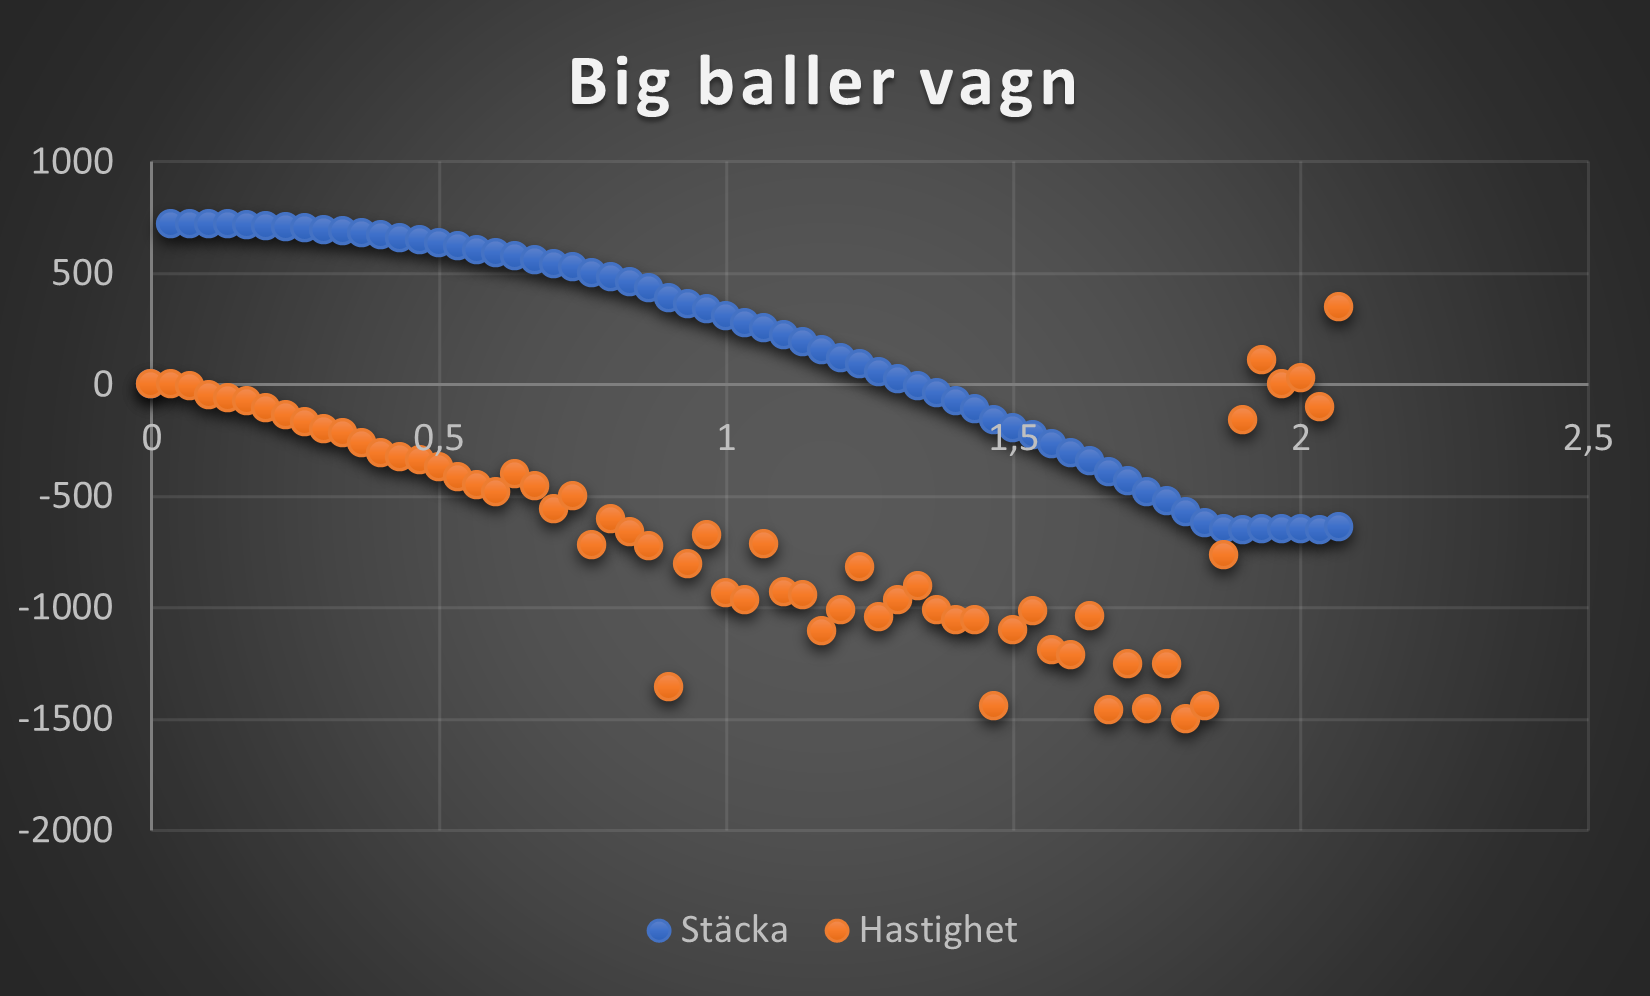
\includegraphics[width=0.8\textwidth]{images/Bild3.png}
            \caption{Graf av med hastighet vid sträcka}
            \label{fig:Bild3}
        \end{figure}
        
    \newpage
	\section{Analys och beräkning}


    Informationen man får av programmet importerades till excel där man räknar ut medelhastigheten med hjälp av formeln.
    \begin{equation}
        v_m = \frac{\Delta s}{\Delta t}
    \end{equation}
    
    \section{Slutsats och resultat} 
        Resultated var väldigt kringelkrokigt eftersom att jag eller alvin gjorde dnågot fel vi uträkningen av sträcka hastighet och acceleration för att graferna visar att allting händer negativt eller i fallet med accelerationen så ser det ut som om det kan ha varit något som hände i star wars. Hade vi gjort om denna lab hade mätningarna gjorts mer noggrant dessutom hade beräkningarna i excel gjorts mer ordentligt så att allt inte går negativt.
\begin{figure}[!h]
	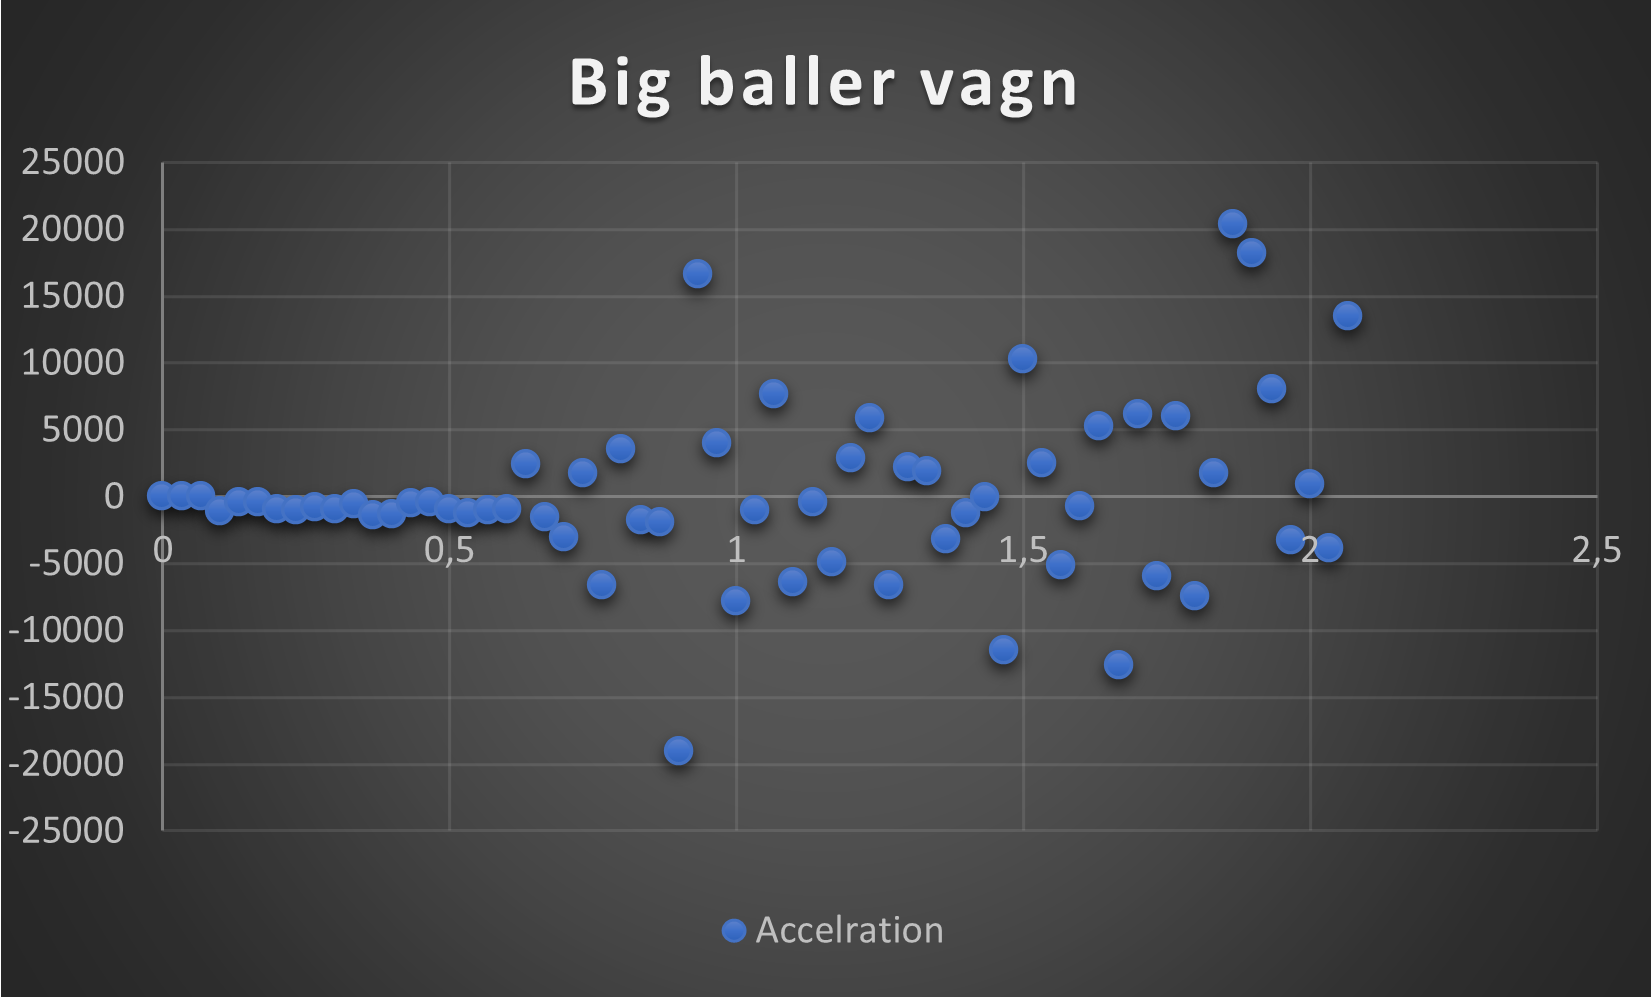
\includegraphics[width=0.8\textwidth]{images/Bild2.png}
	\caption{Graf av acceleration till funktionen tid}
	\label{fig:Bild2}
\end{figure}
\begin{figure}[!h]
	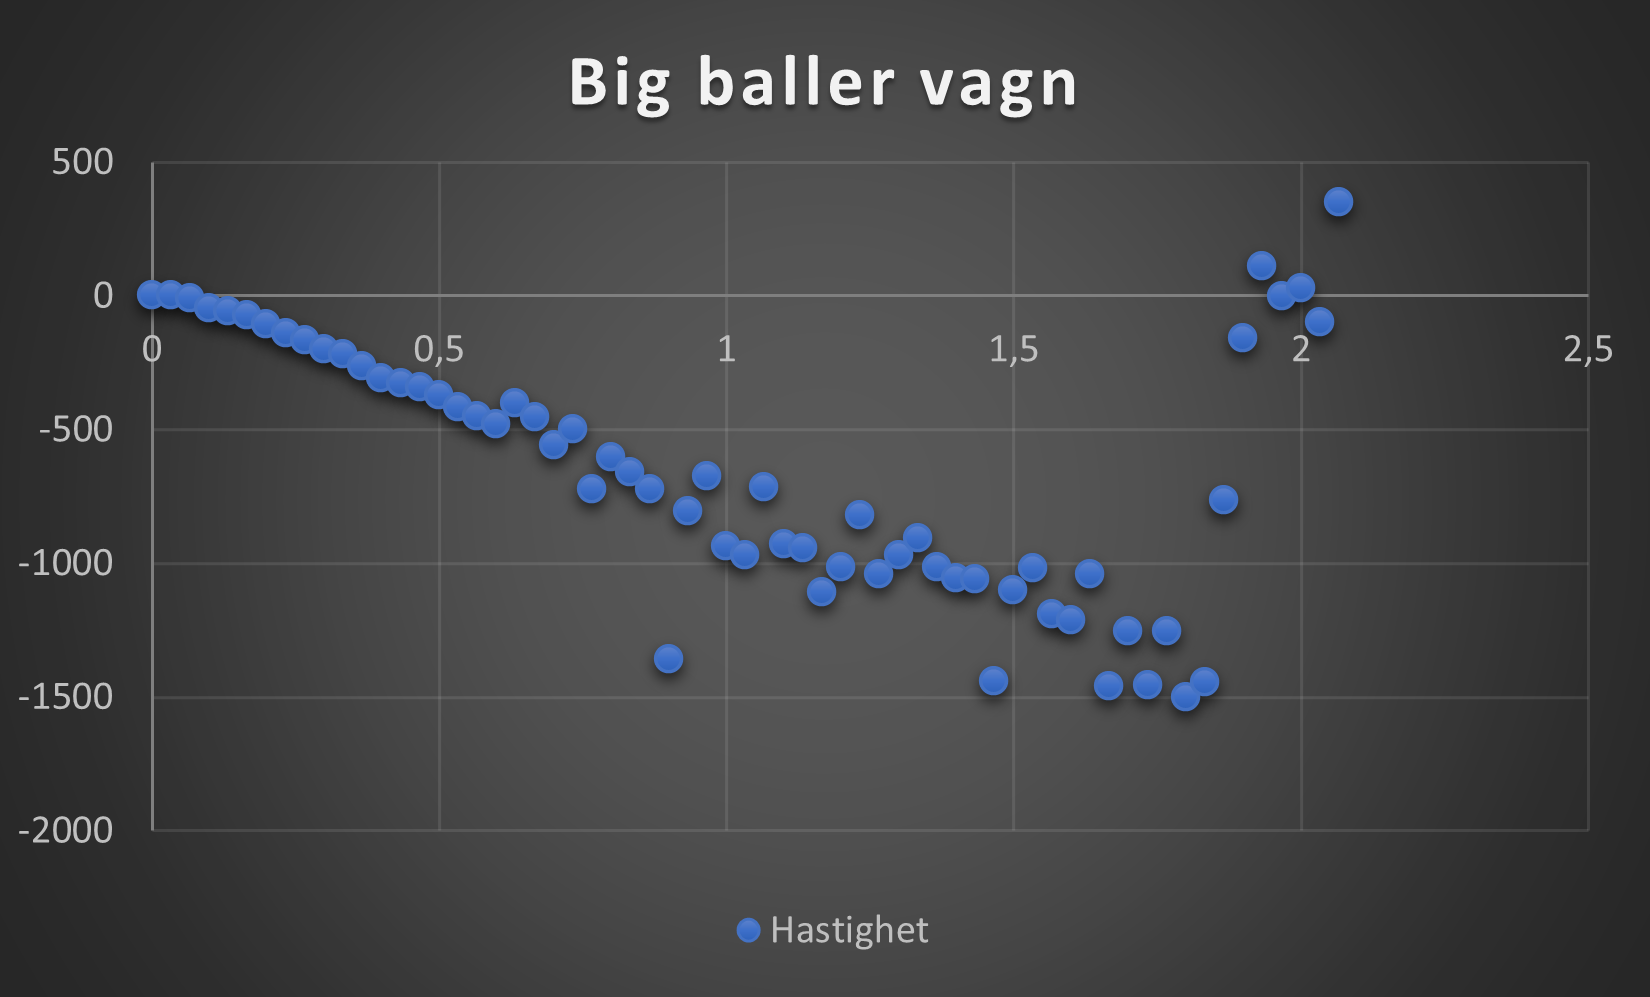
\includegraphics[width=0.8\textwidth]{images/Bild1.png}
	\caption{Graf av hastighet till funktionen tid}
	\label{fig:Bild1}
\end{figure}
    \section{Diskussion} 
    Jag tror nog att allt kunde gjorts mer noggrant men eftersom att man blev förbannad över att mätningsprogrammet inte ville funka först blev man nöjd så fort man fick någonting ur det. Resultatet vi fick är nog heller inte så värst trovärdigt för att jag tor inte att en sträcka kan bli negativ, en hastighet bli negativ eller en acceleration bli negativ.

    
    \printbibliography

\end{document}

